\documentclass[12pt]{report}

% Packages
\usepackage[utf8]{inputenc}  % Encoding
\usepackage{amsmath}         % Math symbols
\usepackage{amsthm}
\usepackage{amssymb}         % More math symbols
\usepackage{mathrsfs}
\usepackage{tikz}
\usepackage{graphicx}        % For including graphics
\usepackage{hyperref}        % For hyperlinks
\usepackage{geometry}        % Adjust page margins
\usepackage{xcolor}
\geometry{a4paper, margin=1in}
\newtheorem{theorem}{Theorem}[section]   
\newtheorem{corollary}{Corollary}[section] 
\newtheorem{lemma}{Lemma}[section]         
\newtheorem{definition}{Definition}[section] 
\newtheorem{proposition}{Proposition}[section]
\newtheorem{example}{example}[section]
\newtheorem{remark}{Remark}[section]
\newtheorem{examples}{Examples}[section]
% Title Page
\title{Calculus of Variations}
\author{Yutan Zhang\\ \texttt{yz7209@nyu.edu}}
\date{\today}
\begin{document}
\maketitle
\tableofcontents
\newpage
\section{Lecture 1, Jan 22, 2025}
\begin{definition}[Calculus of Variations]
Calculus of variations is the collection of methods and techniques used to solve/understand a class of minimization problems for functionals. \footnote{A functional is a function of functions.}
\end{definition}
\subsection{Model Problem (One-variable functions)} 
\hspace*{1.5em}For a function \(u:(a, b) \to \mathbb{R}\), define the integral \(I(u) = \int_a^b f(x, u(x), u'(x)) dx\), where \(f: (a, b) \times \mathbb{R} \times \mathbb{R} \to \mathbb{R}\) is a given continuous function. 

Our goal is to find a function \(\overline{u} \in \Xi\), such that \[I(\overline{u}) \leq I(u)\] for all \(u \in \Xi\).  \footnote{\(\Xi\) is a class of admissible functions. } 

Equivalently, it is to find \(\overline{u} \in \Xi\), such that
\begin{equation}
I(\overline{u}) = \text{min}_{u \in \Xi} I(u). \tag{1}
\end{equation}

\(\overline{u}\) is called a minimizer of  (1). 
\begin{examples}
\begin{enumerate}
    \item Optics. By Fermat's principle, the path of light between two points through a medium is the path that requires minimum travel time. 
\begin{center}
    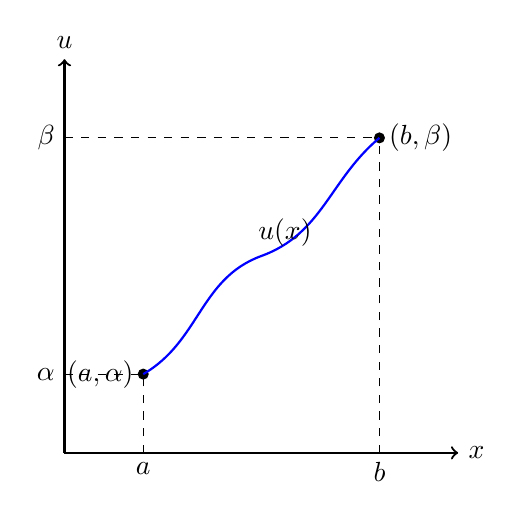
\begin{tikzpicture}
        % Axes
        \draw[thick, ->] (0,0) -- (5,0) node[right] {$x$};
        \draw[thick, ->] (0,0) -- (0,5) node[above] {$u$};

        % Points and labels
        \fill (1,1) circle (2pt) node[left] {$(a,\alpha)$};
        \fill (4,4) circle (2pt) node[right] {$(b,\beta)$};
        
        % Function curve
        \draw[thick, blue] (1,1) to[out=30, in=200] (2.5,2.5) to[out=20, in=220] (4,4);
        \node[black] at (2.8,2.8) {$u(x)$};
        
        % Tick marks and labels
        \draw[dashed] (1,0) -- (1,1);
        \draw[dashed] (4,0) -- (4,4);
        \draw[dashed] (0,1) -- (1,1);
        \draw[dashed] (0,4) -- (4,4);

        \node[below] at (1,0) {$a$};
        \node[below] at (4,0) {$b$};
        \node[left] at (0,1) {$\alpha$};
        \node[left] at (0,4) {$\beta$};

    \end{tikzpicture}
\end{center}
The above graph is an example of the shape of light paths between the two points \((a, \alpha)\) and \((b, \beta)\), where \(u: (a,b) \to \mathbb{R}\) is one of the functions with \(u(a) = \alpha\) and \(u(b) = \beta\). 

To minimize travel time \(T(u(x))\), where 
\begin{equation}
T(u(x)) = \int (\frac{1}{\text{rate}}) d (\text{arc length}) = \int_a^b \frac{1}{v(x, u)} ds = \int_a^b \frac{n(x, u)}{c} \sqrt{1+(u'(x))^2} dx \tag{2}
\end{equation}
Our problem statement is as follows:
\[\Xi = \{u \in C^1[a, b]|u(a) = \alpha, u(b) = \beta\}\]
\[I(u) = \frac{1}{c} \int_a^b n(x, u) \sqrt{1+(u'(x))^2}\]
We aim to find \(\overline{u} \in \Xi\), such that \(I(\overline{u} = \text{min}_{u \in \Xi} I(u)\). 

\item Brachistochrone problem: We aim to find the path \(u(x)\) under which a particle of mass \(m\) falls under gravity, such that the travel time is a minimum. 
\begin{center}
    \begin{tikzpicture}
        % Axes
        \draw[thick, ->] (0,0) -- (5,0) node[right] {$x$};
        \draw[thick, ->] (0,5) -- (0,-1) node[left] {$u$};

        % Points and labels
        \fill (1,4) circle (2pt) node[left] {$(0,0)$};
        \fill (4,1) circle (2pt) node[right] {$(b,\beta)$};
        
        % Function curve
        \draw[thick, green] (1,4) to[out=-60, in=180] (4,1);
        \node[green] at (2.8,2.5) {$u(x)$};
        
        % Tick marks and labels
        \draw[dashed] (4,0) -- (4,1);
        \draw[dashed] (0,1) -- (4,1);

        \node[below] at (4,0) {$b$};
        \node[left] at (0,1) {$\beta$};

    \end{tikzpicture}
\end{center}
For a mass starting at \((0, 0)\), sliding along a wire with shape \(u(x)\) until it reaches the point \((b, \beta)\). 

Travel time is as follows: 
\begin{equation}
T(u(x) = \int_a^b \frac{1}{v(x)} d(\text{arc length}) = \int_a^b \frac{1}{v(x)} \sqrt{1+(u'(x))^2}dx \tag{3}
\end{equation}
In this case, we can find velocity through energy, i.e., 
\[v = \sqrt{-2gu}\]
Therefore, 
\begin{equation}
T(u(x)) = \int_a^b \sqrt{\frac{1+(u'(x))^2}{-2gu(x)}} dx \tag{4}
\end{equation}
And the problem statement of this problem would become
\[\Xi = \{u \in C^1[a, b]|u(0) = 0. u'(b) = 0\}\]
\[I(u) = \int_a^b \sqrt{\frac{1+(u'(x))^2}{-2gu(x)}} dx\]
Our goal is to find \(\overline{u} \in \Xi\), such that \[I(\overline{u}) = \text{min}_{u \in \Xi} I(u).\]

\item Minimum Surface of Revolution: Determine all surfaces of revolution with fixed end points that minimize area. 

For a curve in the shape \(u(x)\), with endpoints \((a, \alpha)\) and \((b, \beta)\), such that \(u(a) = \alpha\) and \(u(b) = \beta\), the surface formed by rotating the curve along the x-axis is calculated by 
\begin{equation}
A(u) = 2\pi\int_a^b u(x) \sqrt{1+(u'(x))^2}dx \tag{5}
\end{equation}
\begin{figure}
    \centering
    \includegraphics[width=0.5\linewidth]{3D_surface_of_revolution.png}
\end{figure}
Problem statement in this case is as follows:
\[\Xi = \{u \in C^1[a, b]|u(a) = \alpha, u(b) = \beta, u(x) > 0\}\]
\[I(u) = 2\pi\int_a^b u(x) \sqrt{1+(u'(x))^2}dx\]
We aim to find \(\overline{u} \in \Xi\) such that \[I(\overline{u}) = \text{min}_{u \in \Xi} I(u).\]
\item Higher dimensions. The integral to minimize is
\[
I(u) := \int_\Omega f(\vec{x}, u(\vec{x}), \nabla u(\vec{x})) \, d\vec{x},
\]
where $f : \Omega \times \mathbb{R} \times \mathbb{R}^d \to \mathbb{R}$ is a continuous function.

Our goal is to find a function $\bar{u} \in \Xi$ such that
\[
I(\bar{u}) \leq I(u) \quad \text{for all } u \in \Xi.
\]

Equivalently, it is to find $\bar{u} \in \Xi$ such that
\[
I(\bar{u}) = \min_{u \in \Xi} I(u).
\tag{6}
\]

\textit{Notes:}
\begin{itemize}
    \item $\int_\Omega$ can represent a double or triple integral.
    \item $d\vec{x}$ corresponds to $dx_1 dx_2$ or $dx_1 dx_2 dx_3$ depending on the context.
\end{itemize}

\item Dirichlet integral. \[
\Xi = \left\{
u, \nabla u \text{ square integrable} \; : \;
u(\vec{x}) = g(\vec{x}) \text{ for all } \vec{x} \in \partial \Omega
\right\},
\]
where $g$ is a given function.

\[
I(u) = \int_\Omega \frac{1}{2} |\nabla u(\vec{x})|^2 \, d\vec{x}.
\]
Our goal is to find \(\bar{u} \in \Xi\) such that \(I(\bar{u}) = \min_{u \in \Xi} I(u).\)

Note: In this case, we have 
\[
f(\vec{x}, u, \vec{\xi}) = \frac{1}{2} |\vec{\xi}|^2
\]

\item Minimum Surfaces. 

For a Surface given by \[
S = \{ (\vec{x}, u(\vec{x})) \mid \vec{x} \in \Omega \},
\]
its area is calculated as \[
A = \int_{\Omega} \sqrt{1 + |\nabla u(\vec{x})|^2} \, d\vec{x}.
\]

Suppose \(\Gamma\) is a closed curve in \(\mathbb{R}^{n+1}\), our goal is to find all surfaces \( \Sigma \) in \( \mathbb{R}^{n+1} \) with boundary \( \partial \Sigma = \Gamma \), such that the area of \( \Sigma \) is minimized.

Note: In reality, the film formed by dipping a wire in soapy water is a minimal surface. 

The problem statement in this case is as follows:
\[
\Xi = \left\{ u | u \text{ integrable, } u(\vec{x}) = g(\vec{x}) \text{ for all } \vec{x} \in \partial \Omega \text{ for the given function } g \right\}
\]
\[
\mathcal{I}(u) = \int_{\Omega} \sqrt{1 + |\nabla u(x)|^2} \, dx.
\]

Our goal is to find \( \bar{u} \in \Xi \), such that
\[
\mathcal{I}(\bar{u}) = \min_{u \in \Xi} \mathcal{I}(u).
\]

Note: In this case, we have
\[
f(x, u, \xi) = \sqrt{1 + |\xi|^2}
\]

\item Isoperimetric Inequality. 
Let \( A \) be a bounded region in \( \mathbb{R}^2 \) whose boundary \( \partial A \) is a sufficiently regular closed curve (meaning it does not oscillate or bend too much and does not cross over itself).

\[
L(\partial A) := \text{length of the boundary } \partial A.
\]
\[
M(A) := \text{area of } A.
\]

\textit{Isoperimetric Inequality Statement:}
\[
[L(\partial A)]^2 - 4\pi M(A) \geq 0, \quad \text{for all } A.
\]
The inequality becomes an equality if and only if \( A \) is a disk (i.e., \( \partial A \) is a circle).

We can turn this into a minimization problem as follows
\[
\text{Parameterize } \partial A: \quad \partial A = \left\{ \vec{u}(t) = (x(t), y(t)) \mid t \in [a, b] \right\}.
\]

\[
L(\partial A) = \int_{a}^{b} \sqrt{(x'(t))^2 + (y'(t))^2} \, dt := L(\vec{u}).
\]

\[
M(A) = \frac{1}{2} \int_{a}^{b} \left[ x(t) y'(t) - x'(t) y(t) \right] \, dt := M(\vec{u}).
\] \footnote{This area formula is derived from Green's Theorem. }

Admissible functions:
\[
\Xi = \left\{ \vec{u} \in C^1([a,b]) \mid \vec{u}(a) = \vec{u}(b), \, M(\vec{u}) = 1 \right\}.
\]
Our goal is to show that 
\[
\min_{\vec{u} \in \Xi} L(\vec{u}) = \sqrt{4\pi}.
\]
This implies the isoperimetric inequality since
\[
L(\vec{v}) \geq \min_{\vec{u} \in \Xi} L(\vec{u}) = \sqrt{4\pi}
\]
\[
\Rightarrow (L(\vec{v}))^2 \geq 4\pi = 4\pi M(\vec{v})
\]
for all \( M(\vec{v}) = 1 \) with \( \vec{v} \in \Xi \).



\end{enumerate}
\end{examples}
\section{Lecture 2, Jan 27, 2025}
\subsection{Definition of \(C^k\)}
\[
C^k(\Omega) = \left\{ u : \Omega \to \mathbb{R} : u \text{ and all its partial derivatives up to} \right.
\]
\[
\left. \text{and including order } k \text{ are in } C^0(\Omega) \right\}.
\]
The sets \( C^k(\Omega) \) are function spaces.
\subsection{Spaces of continuous functions} 
\[\|u\|_{C^0(\Omega)} = \text{sup}_{x \in \Omega} |u(x)|\]
\[\|f\|_{C^k (\Omega)} = \sum_{|\alpha| \leq k} \sup_{x \in \Omega} |D^\alpha f(x)|
 \]
\subsection{Convex Analysis in Higher Dimensions}
\hspace*{1.5em}For \(\Omega \subseteq \mathbb{R}^n\), \(f: \Omega \to \mathbb{R}\) is convex if for any pair \(\vec{x}, \vec{y} \in \Omega\), and every \(\lambda \in [0, 1]\), we have \[f(\lambda \vec{x} + (1-\lambda)\vec{y}) \leq \lambda f(\vec{x}) + (1-\lambda) f(\vec{y}). \] 
If \(f \in C^1\), $f$ is convex if 
\[
f(\vec{x}) \geq f(\vec{y}) + \nabla f(\vec{y}) \cdot (\vec{x} - \vec{y})
\]
for all $\vec{x}, \vec{y} \in \Omega$. 

Suppose $f \in C^2(\Omega)$. $f$ is convex if the Hessian matrix
\[
\nabla^2 u(\vec{x}) := 
\begin{bmatrix}
\frac{\partial^2 u}{\partial x_1^2} & \frac{\partial^2 u}{\partial x_1 \partial x_2} & \cdots & \frac{\partial^2 u}{\partial x_1 \partial x_n} \\
\frac{\partial^2 u}{\partial x_2 \partial x_1} & \frac{\partial^2 u}{\partial x_2^2} & \cdots & \frac{\partial^2 u}{\partial x_2 \partial x_n} \\
\vdots & \vdots & \ddots & \vdots \\
\frac{\partial^2 u}{\partial x_n \partial x_1} & \frac{\partial^2 u}{\partial x_n \partial x_2} & \cdots & \frac{\partial^2 u}{\partial x_n^2}
\end{bmatrix}
\]
is positive semi-definite.

\subsection{Jensen's Inequality}
Let $u : [a, b] \to \mathbb{R}$ be an integrable function.  

Let $f : \mathbb{R} \to \mathbb{R}$ be convex. Then
\[
f\left( \frac{1}{b-a} \int_a^b u(x) \, dx \right) 
\leq 
\frac{1}{b-a} \int_a^b f(u(x)) \, dx.
\]

\subsection{Fundamental Lemma of the Calculus of Variations}
\begin{theorem}
Suppose a function $f : (a, b) \to \mathbb{R}$ is continuous, and suppose that 
\[
\int_a^b f(x) \phi(x) \, dx = 0 \quad \text{for every } \phi \in C^1([a, b]),
\]
with $\phi(a) = 0 = \phi(b)$.  Then $f(x) = 0$ for all $x \in (a, b)$.
\end{theorem}
\subsection{Euler-Lagrange Equation}
Remark: This is a major tool in analyzing problem (P). 

We study 1-dimensional problems for now. Suppose \[I(u) = \int_a^b f(x, u(x), u'(x)) dx,\]where \(f:[a, b] \times \mathbb{R} \times \mathbb{R} \to \mathbb{R}\) belongs to \(C^2([a, b] \times \mathbb{R} \times \mathbb{R})\). 

Recall: This means that all partial derivatives up to and including order 2 exists and are themselves continuous functions. 

Admissible functions are
\begin{equation}
    \Xi = \{ u \in C^1([a,b]) : u(a) = \alpha, u(b) = \beta \}.
\end{equation}

Our goal is to find $ u \in \Xi $ such that
\begin{equation}
    I(u) = \min_{v \in \Xi} I(v). \tag{P}
\end{equation}
\begin{theorem}
Let $ f = f(x,u,\zeta) $ be a $ C^2([a,b] \times \mathbb{R} \times \mathbb{R}) $ function.

Suppose problem (P) has a minimizer $ u \in \Xi \cap C^2([a,b]) $. Then $ u $ satisfies
\begin{equation}
    \frac{d}{dx} \left[ \frac{\partial f}{\partial \zeta} (x, u(x), u'(x)) \right] = \frac{\partial f}{\partial u} (x, u(x), u'(x)) \quad \text{for all } x \in [a,b]. \tag{E}
\end{equation}
Differentiating the left-hand side, we get
\begin{align*}
    \frac{\partial^2 f}{\partial x \partial s} (x, u(x), u'(x)) &+ \frac{\partial^2 f}{\partial u \partial s} (x, u(x), u'(x)) \cdot \frac{du}{dx} \\
    &+ \frac{\partial^2 f}{\partial s^2} (x, u(x), u'(x)) \cdot \frac{d^2 u}{dx^2} = \frac{\partial f}{\partial u} (x, u(x), u'(x)).
\end{align*}

\textcolor{purple}{(E) is called the Euler-Lagrange Equation associated to problem (P)}.
\end{theorem}
Since $u$ is a minimizer, we have
\begin{equation}
    I(u) \leq I(v) \quad \text{for all } v \in \Xi.
\end{equation}
Recall the space of admissible functions
\begin{equation}
    \Xi = \left\{ u \in C^1([a,b]) : u(a) = \alpha, u(b) = \beta \right\}.
\end{equation}
\begin{proof}
Let $w \in C^1([a,b])$ be arbitrary with $w(a) = 0$ and $w(b) = 0$. Let $h \in \mathbb{R}$ be arbitrary. Then the function $u + hw$ belongs to $\Xi$ since
\begin{align*}
    u(a) + hw(a) &= \alpha, \\
    u(b) + hw(b) &= \beta.
\end{align*}
Thus, for any $h \in \mathbb{R}$, we obtain
\begin{equation}
    I(u) \leq I(u + hw).
\end{equation}
Define the function
\begin{equation}
    G(h) := I(u + hw), \quad \text{for } h \in \mathbb{R}.
\end{equation}
Since $G$ has a local minimum at $h = 0$, we conclude that
\begin{equation}
    G'(0) = 0.
\end{equation}
This implies
\begin{equation}
    \left. \frac{d}{dh} I(u + hw) \right|_{h=0} = 0.
\end{equation}
Computing the derivative, we get
\begin{align*}
    \frac{d}{dh} I(u + hw) &= \int_{a}^{b} \frac{d}{dh} \left[ f(x, u + hw, u' + hw') \right] dx \\
    &= \int_{a}^{b} \left[ \frac{\partial f}{\partial u} (x, u + hw, u' + hw') \cdot w 
    + \frac{\partial f}{\partial \zeta} (x, u + hw, u' + hw') \cdot w' \right] dx.
\end{align*}
Evaluating at $h=0$, we get
\begin{equation}
    \int_{a}^{b} \left[ \frac{\partial f}{\partial u} (x, u, u') w + \frac{\partial f}{\partial \zeta} (x, u, u') w' \right] dx = 0.
\end{equation}
By integration by parts, we have
\[\frac{d}{dx}[w(x)\frac{\partial f}{\partial u'}(x, u(x), u'(x))] = w'\frac{\partial f}{\partial u'}(x, u(x), u'(x)) + w\frac{d}{dx}[\frac{\partial f}{\partial u'}(x, u(x), u'(x))]\]
which implies 
\[\int_a^b \frac{d}{dx}[\frac{\partial f}{\partial u'}(x, u(x), u'(x))]dx =w(x)\frac{\partial f}{\partial u'} |_{x = a}^{x = b} = \int_a^b (w'\frac{\partial f}{\partial u'} + w\frac{d}{dx}[\frac{\partial f}{\partial u'}])dx\]
Since \(w(a) = w(b) = 0\), boundary terms vanish. Then we have 
\[\int_a^b w(x)\frac{\partial f}{\partial u} dx = \int_a^b w(x)\frac{d}{dx}[\frac{\partial f}{\partial u'}] dx\]
for arbitrary \(w\). Therefore, by Fundamental Lemma of the Calculus of Variations, we obtain the Euler-Lagrange equation
\[
    \frac{d}{dx} \left( \frac{\partial f}{\partial u'} \right) - \frac{\partial f}{\partial u} = 0.\]
\end{proof}
Remark: If \(u\) is a minimizer and \(u \in C^2\), \(u\) solves (P). 

However, the converse does not hold. in general, if \(f\) is convex in the variables \((u, \zeta)\), then yes. 
\begin{examples}
\begin{enumerate}
    \item \[f(x, u(x), u'(x)) = f(u'(x))\]
Then
\[
\frac{d}{dx} \left[ \frac{\partial f}{\partial \zeta}(\bar{u}(x)) \right] = 0 \implies \frac{\partial f}{\partial \zeta}(\bar{u}(x)) = \text{constant}.
\]

Consider the linear function

\[
\bar{u}(x) = \frac{\beta - \alpha}{b - a}(x - a) + \alpha.
\]

\[
\bar{u}(a) = \alpha, \quad \bar{u}(b) = \beta \implies \bar{u} \in \Xi.
\]

Further,

\[
\bar{u}'(x) = \frac{\beta - \alpha}{b - a} = \text{constant}, \quad \text{so} \quad \frac{\partial f}{\partial \zeta}\left(\frac{\beta - \alpha}{b - a}\right) = \text{constant}.
\]

However, $\bar{u}$ is not always a minimizer of $(P)$.
\item Following the previous example, here we have \(f\) convex.

Recall: This means \( f''(u') \geq 0 \) for all \( u' \). In this case, \( \bar{u} \) is indeed a minimizer of (P).

By Jensen’s Inequality,
\[
\frac{1}{b-a} I(u) =
\]
\[
\frac{1}{b-a} \int_{a}^{b} f(u' (x)) dx \geq f \left( \frac{1}{b-a} \int_{a}^{b} u' (x) dx \right)
\]
\[
= f \left( \frac{u(b) - u(a)}{b-a} \right) = f \left( \frac{\beta - 2}{b-a} \right) = f \left( \bar{u}^i (x) \right)
\]
\[
= \frac{1}{b-a} \int_{a}^{b} f(\bar{u}^i (x)) dx = \frac{1}{b-a} I(\bar{u})
\]
\[
\Rightarrow I(u) \geq I(\bar{u}) \quad \text{for all } u \in \Xi, \text{ so } \bar{u} \text{ is a minimizer.}
\]
\item Here \( f \) is not convex.

In this case, (P) has no minimizer in general.  
For example, take \( a = 0 \), \( b = 1 \), and let \( f(\xi) = e^{-\xi^2} \).  

Then  
\[
I(u) = \int_{0}^{1} e^{-(u'(x))^2} dx.
\]

Clearly, no function \( u \in \Xi \) can satisfy the equality  
\[
\int_{0}^{1} e^{-(u'(x))^2} dx.
\]

However, there exists a sequence of functions \( \{ u_n \} \) belonging to \( \Xi \) such that  
\( I(u_n) \to 0 \) as \( n \to \infty \).  

An example would be  
\[
u_n (x) := n \left( x - \frac{1}{2} \right)^2 - \frac{n}{4}, \quad u_n: [0,1] \to \mathbb{R}
\]
for all \( n \in \mathbb{N} \). Then  
\[
u_n'(x) = 2n \left( x - \frac{1}{2} \right),
\]
and  

\[
I(u_n) = \int_{0}^{1} e^{-4n^2 (x - \frac{1}{2})^2} dx.
\]

By change of variables, let \( y = 2n (x - \frac{1}{2}) \), then we have  

\[
I(u_n) = \frac{1}{2n} \int_{-n}^{n} e^{-y^2} dy = \lim_{n \to \infty} \frac{1}{2n} \int_{-\infty}^{+\infty} e^{-y^2} dy.
\]

\[
= \lim_{n \to \infty} \frac{\sqrt{\pi}}{2n} = 0.
\]

Therefore, \( I \) has no minimizer in \( \Xi \).
\item 
In this case, $f(x, u, u') = f(u, u')$, which makes it more difficult than the previous case.



Recall that the Euler--Lagrange Equation is

\[
\frac{d}{dx} \left[ \frac{\partial f}{\partial u'}(u(x), u'(x)) \right] = \frac{\partial f}{\partial u}(u(x), u'(x)) \tag{E}.
\]

We shall convert (E) into another more useful form.

First Integral Form of Euler--Lagrange Equation:

Consider
\[
\frac{d}{dx} \left[ f(u(x), u'(x)) - u'(x) \frac{\partial f}{\partial u'}(u(x), u'(x)) \right].
\]

\[
= \frac{\partial f}{\partial u} u' + \frac{\partial f}{\partial u'} u'' - \left( u'' \frac{\partial f}{\partial u'} + u' \frac{d}{dx} \left( \frac{\partial f}{\partial u'} \right) \right)
\]
By Euler-Lagrange equation, we have
\[\frac{d}{dx}\frac{\partial f}{\partial \zeta} = \frac{\partial f}{\partial u}\]
Therefore, we get 
\[
\frac{d}{dx} \left[ f(u(x), u'(x)) - u'(x) \frac{\partial f}{\partial u'}(u(x), u'(x)) \right] = 0
\]
which means \[\left[ f(u(x), u'(x)) - u'(x) \frac{\partial f}{\partial u'}(u(x), u'(x)) \right] = \text{constant}\]
\item Brachistochrone problem.

Recall:
\begin{align*}
    \Xi &= \{ u \in C^1[0,b] \mid u(0) = 0, u(1)(b) = 0 \} \\
    f(x,u,u') &= \frac{\sqrt{1 + (u')^2}}{-2g u} \\
    I(u) &= \int_0^b \frac{\sqrt{1 + (u'(x))^2}}{-2g u(x)} \ dx
\end{align*}

By the previous discussion, the first integral form of the Euler-Lagrange equation is in the form

\begin{align*}
    \frac{\sqrt{1 + (u')^2}}{-2g u} - u' \left( \frac{u'}{-2g u (1 + (u')^2)} \right) &= \text{constant} \\
    \frac{1}{\sqrt{-2g u} \sqrt{1 + (u')^2}} &= \text{constant} \\
    \implies (1 + (u')^2)(-u(x)) &= \mu,
\end{align*}
where $\mu > 0$ is some constant.

Solve this ODE: 

\(u(x)\) = curve traced by \((u(t), x(t))\), then \[u'(x) = \frac{\frac{du}{dt}}{\frac{dx}{dt}}\]Therefore, \[\frac{(\frac{du}{dt})^2}{(\frac{dx}{dt})^2} = \frac{\mu}{-u(t)} - 1 = \frac{\mu + u(t)}{-u(t)}\]
\[
    \left( \frac{dx}{dt} \right)^2 = \frac{-u(t)}{\mu + u(t)} \left( \frac{du}{dt} \right)^2
\]
\[
    \frac{dx}{dt} = -\sqrt{\frac{-u(t)}{\mu + u(t)}} \frac{du}{dt}.
\]
By integration, we get
\[
    x(t) = - \int \sqrt{\frac{-u(t)}{\mu + u(t)}} \frac{du}{dt}.
\] \footnote{\(\frac{dx}{dt} \geq 0\), \(\frac{du}{dt} \leq 0\), so we choose "-". }
Substituting $ u(t) = -\mu \sin^2(\theta) $ \footnote{\[u(t(\theta)) = -\mu \sin^2{\theta}\]  \[\frac{du(t(\theta))}{d\theta} = u'(t) \frac{dt}{d\theta}\] \[\frac{du}{d\theta} = -2\mu \sin{\theta} \cos{\theta}\] \[du = u'(t) \frac{dt}{d\theta} d\theta = -2\mu \sin{\theta} \cos{\theta} d\theta\]}, we get \(u'(t) dt = -2\mu \sin{\theta} \cos{\theta} d\theta\), then
\[
    x = 2\mu \int \frac{\sin^2(\theta)}{1 - \sin^2(\theta)} \sin(\theta) \cos(\theta) \, d\theta
\] \[= 2\mu \int \sin^2{\theta} d\theta\] \[= \mu \int (1-\cos{2\theta}) d\theta = \mu (\theta -\frac{1}{2} \sin{2\theta}) + C\]
Using the substitution $ \phi = 2\theta $, we arrive at
\[
    x(\phi) = \frac{\mu}{2} (\phi - \sin \phi) + C, \quad u(\phi) = -\frac{\mu}{2} (1 - \cos \phi).
\]
Using boundary conditions, we solve for $\mu$ and \(C\)
\[
    b = x(\pi) = \frac{\pi \mu}{2} \Rightarrow \mu = \frac{2b}{\pi}
\] \[x(0) = 0, u(0) = 0 \Rightarrow C = 0\]
Thus, our final solution is
\[
    x(\phi) = \frac{b}{\pi} (\phi - \sin \phi), \quad u(\phi) = -\frac{b}{\pi} (1 - \cos \phi), \quad 0 \leq \phi \leq \pi.
\]
This is a \textbf{cycloid curve}.
\item Minimal surface of Revolution

\[
X = \left\{ u \in C^1[a,b], \quad u(a) = \alpha, \quad u(b) = \beta, \quad u(x) > 0 \right\}.
\]

\[
\Pi (u) = \int_a^b 2\pi u \sqrt{1+ (u')^2} \,dx.
\]

\[
f(x, u, u_x) = 2\pi u \sqrt{1+ (u')^2}
\]

\[
\frac{\partial f}{\partial  u'} = \frac{2\pi u (-2 u')}{\sqrt{1+(u')^2}} = \frac{2\pi u u'}{\sqrt{1+ (u')^2}}.
\]

By Euler-Lagrange Equation, 

\[
\frac{d}{dx} \left( \frac{2\pi u u'}{\sqrt{1+(u')^2}} \right) = 2\pi \sqrt{1+(u')^2}.
\]

By First Integral Form of Euler-Lagrange Equation, 

\[
2\pi u \sqrt{1+(u')^2} -\frac{ 2\pi u (u')^2}{\sqrt{1+(u')^2}} = \text{constant} = \mu.
\]

\[
2\pi u  = \mu \sqrt{1+(u')^2}.
\]

Solve for \( u'(x) \)

\[
\frac{du}{dx} = u'(x) = \sqrt{\left(\frac{2\pi}{\mu} u\right)^2 - 1}.
\]

which is a first-order separable ODE. 

\[
\int \frac{1}{\sqrt{\left(\frac{2\pi}{\mu} u\right)^2 - 1}} \,du = \int dx
\]

\[
x = \frac{\mu}{2\pi} \int \frac{1}{\sqrt{u^2 - \left(\frac{\mu}{2\pi}\right)^2}} \,du
\]

Let \( u = \frac{\mu}{2\pi} \cosh(\theta) \), we get \(
du = \frac{\mu}{2\pi} \sinh(\theta) d\theta
\), so 

\[
x = \frac{\mu}{2\pi} \int \frac{\sinh(\theta)}{\cosh^2(\theta) - 1} d\theta = \frac{\mu}{2\pi} \int d\theta.
\]

\[
x = \frac{\mu}{2\pi} \theta + C.
\]

\[
\theta = \frac{2\pi}{\mu} (x+C).
\]

\[
u = \frac{\mu}{2\pi} \cosh \left(\frac{2\pi}{\mu} (x+C)\right).
\]

(\( C \) is arbitrary.)

Thus,
\[ u(x) = \frac{\mu}{2\pi} \cosh\left(\frac{2\pi}{\mu} (x + c)\right) \]
This is called a catenary.

Obtain \( \mu \) and \( c \) from boundary conditions
\[
\begin{cases}
    u(a) = \alpha \\
    u(b) = \beta
\end{cases}
\Rightarrow
\begin{cases}
    \alpha = \frac{\mu}{2\pi} \cosh\left(\frac{2\pi}{\mu} (a + c)\right), \\
    \beta = \frac{\mu}{2\pi} \cosh\left(\frac{2\pi}{\mu} (b + c)\right).
\end{cases}
\]
Solve for \( \mu \), \( c \).

Example:
\[ a = 1, \quad b = 1, \quad \alpha = \beta = 2. \]

\[ 2 = \frac{\mu}{2\pi} \cosh\left(\frac{2\pi}{\mu} (c + 1)\right) \Rightarrow c = 0. \]

\[ 2 = \frac{\mu}{2\pi} \cosh\left(\frac{2\pi}{\mu} (c + 1)\right). \]

\[ 4\pi = \mu \cosh\left(\frac{2\pi}{\mu}\right). \]

Numerics lead to two roots:
\[ \mu_1 \approx 2.954, \quad \mu_2 \approx 10.661. \]

Which value(s) give the global minimum?

Check:
\[
\begin{aligned}
    u_1(x) &= \frac{\mu_1}{2\pi} \cosh\left(\frac{2\pi}{\mu_1} x\right) \Rightarrow I(u_1) = 22.3878, \\
    u_2(x) &= \frac{\mu_2}{2\pi} \cosh\left(\frac{2\pi}{\mu_2} x\right) \Rightarrow I(u_2) = 23.968.
\end{aligned}
\]
\item Fermat's Principle
We consider the integral
\[ I(u) = \frac{1}{c} \int_a^b n(x,u) \sqrt{1+(u')^2} \, dx. \]

where
\[ f(x,u,s) = \frac{n(x,u)}{c} \sqrt{1+s^2}. \]

By Euler-Lagrange equation, 
\[ \frac{d}{dx} \left[ \frac{\partial}{\partial u'} \left( \frac{n(x,u)}{c} \sqrt{1+(u')^2} \right) \right] = \frac{1}{c} \frac{\partial n}{\partial u} \sqrt{1+(u')^2}. \]

After differentiation, we get
\[ \frac{n(x,u)}{c} u''(x) + \frac{1}{c} \left( \frac{\partial n}{\partial x} (x,u) u'(x) - \frac{\partial n}{\partial u} (x,u) \right) \left( 1+(u'(x))^2 \right) = 0. \]

This is a nonlinear second-order ODE.

\end{enumerate}
\end{examples}
\section{Lecture 3, Jan 29, 2025}
\subsection{Sequences}
Omitted. 
\section{Lecture 4, Feb 3, 2025}
\subsection{\(L^p\) spaces}
Let \(\Omega\) be a region in \(\mathbb{R}^d\), let \( p \in [1, \infty) \).
\begin{definition}
A function \( u: \Omega \to \mathbb{R} \) belongs to \( L^p(\Omega) \) if
\[
\left( \int_{\Omega} |u(x)|^p \, dx \right)^{\frac{1}{p}} < \infty.
\]
\( L^p(\Omega) \) is a Banach space, with norm
\[
\|u\|_{L^p(\Omega)} := \left( \int_{\Omega} |u(x)|^p \, dx \right)^{\frac{1}{p}}.
\]
\end{definition}
For \( p = \infty \), \( L^\infty(\Omega) \) is a Banach space with norm
\[
\|u\|_{L^\infty(\Omega)} = \operatorname{ess\,sup}_{x \in \Omega} |u(x)|.
\]

Remark: Essential Supremum:

\(\operatorname{ess\,sup}\) = "essential supremum"  
Supremum but for functions defined \emph{almost everywhere}.  

\(\operatorname{ess\,sup} = \sup\) for continuous functions.
\begin{theorem}[Hölder Inequality]
Let \( p \in (1, \infty] \) and let \( p' = \frac{p}{p-1} \) (equivalently, \( \frac{1}{p} + \frac{1}{p'} = 1 \)).

If \( u \in L^p(\Omega) \) and \( v \in L^{p'}(\Omega) \), then \( uv \in L^1(\Omega) \) with
\[
\int_{\Omega} |u(x) v(x)| \, dx \leq \|u\|_{L^p(\Omega)} \|v\|_{L^{p'}(\Omega)}.
\]
\end{theorem}
\begin{corollary}
When \( p = 2 \), \( p' = 2 \) and
\[
\int_{\Omega} |u(x) v(x)| \, dx \leq \|u\|_{L^2(\Omega)} \|v\|_{L^2(\Omega)}.
\]
(This is the \textit{Cauchy-Schwartz inequality}.)
\end{corollary}
When \( p = 1 \), \( p' = \infty \) (and vice versa).
\begin{theorem}[Minkowski Inequality / Triangle Inequality in \( L^p \)]
\[
\|u + v\|_{L^p(\Omega)} \leq \|u\|_{L^p(\Omega)} + \|v\|_{L^p(\Omega)}.
\]
\end{theorem}
\begin{theorem}[Density of Smooth Functions]
Let \( 1 \leq p < \infty \). The functions in \( C_c^\infty(\Omega) \), the \( C^\infty \) functions with compact support on \( \Omega \), are \textit{dense} in \( L^p(\Omega) \).  

This means that for \( u \in L^p(\Omega) \), there exists a sequence \( \{ u_n \} \) belonging to \( C_c^\infty(\Omega) \) such that
\[
\lim_{n \to \infty} \| u_n - u \|_{L^p(\Omega)} = 0.
\]
\end{theorem}
\subsection{Sequences and Convergence of functions in \(L^p (\Omega)\)}
\begin{definition}[Strong Convergence]
A sequence \( \{ u_n \} \) of functions in \( L^p(\Omega) \) is said to \textit{converge}, or \textit{strongly converge}, to \( u \in L^p(\Omega) \) if
\[
\lim_{n \to \infty} \| u_n - u \|_{L^p(\Omega)} = 0.
\]
We write: \( u_n \to u \) in \( L^p(\Omega) \).
\end{definition}
\begin{definition}[Weak Convergence]
If \( 1 \leq p < \infty \), a sequence \( \{ u_n \} \) of functions in \( L^p(\Omega) \) \textit{weakly} converges to \( u \in L^p(\Omega) \) if
\[
\lim_{n \to \infty} \int_{\Omega} ( u_n(x) - u(x) ) \varphi(x) \, dx = 0, \quad \forall \varphi \in L^{p'}(\Omega).
\]
We write: \( u_n \rightharpoonup u \) in \( L^p(\Omega) \).\footnote{\(\frac{1}{p} + \frac{1}{p'} = 1\) here. }
\end{definition}
If \( p = \infty \), a sequence \( \{ u_n \} \) of functions in \( L^\infty(\Omega) \) \textit{weak-* converges} to \( u \in L^\infty(\Omega) \) if
\[
\lim_{n \to \infty} \int_{\Omega} ( u_n(x) - u(x) ) \varphi(x) \, dx = 0, \quad \forall \varphi \in L^1(\Omega).
\]
We write: \( u_n \overset{*}{\rightharpoonup} u \) in \( L^\infty(\Omega) \).

\section{Lecture 5, Feb 5, 2025}

\subsection{Another Form of the Poincaré Inequality}

Define 
\[
u_\Omega := \frac{1}{|\Omega|} \int_{\Omega} u(x) \,dx.
\]
$u_\Omega$ is a real number (recall that $\int_{\Omega} 1 dx < \infty$). 

Then there exists a constant $C > 0$ depending only on $\Omega$ and $p$ such that
\[
\| u - u_\Omega \|_{L^p(\Omega)} \leq C \| \nabla u \|_{L^p(\Omega)}, \quad \forall u \in W^{1,p}(\Omega).
\]

\subsection{A Third Form of the Poincaré Inequality}

Let $\Omega$ be bounded, and let $1 \leq p \leq \infty$. Let $u \in W^{1,p}(\Omega)$. 

Suppose $g \in W^{1,p}(\Omega)$ such that
\[
u(x) - g(x) \in W^{1,p}_0(\Omega).
\]
\textcolor{red}{This means that $u = g$ on $\partial \Omega$.}

Then there exist $\gamma, \gamma_0, \gamma_2 > 0$ depending only on $p$ and $\Omega$ such that
\[
\gamma \| u \|_{W^{1,p}(\Omega)} = \gamma_1 \| g \|_{W^{1,p}(\Omega)} \leq \| \nabla u \|_{L^p(\Omega)}.
\]

\subsection{Proof}

For simplicity, let $d = 1$ and $\Omega = (a,b)$. 

$u \in W^{1,p}_0(a,b)$ means $u(a) = 0 = u(b)$. 
\section{Lecture 6, Feb 10, 2025}

\section{Lecture 7, Feb 12, 2025}


\end{document}
